\chapter{Sharing medical images}
\label{sec:imaging}
%\label{sec:medicalapp}
This chapter introduces acquiring, storing and sharing digital medical images and related metadata within hospital or healthcare provider and among them and research institution.

%are covered in section \ref{sec:introimages}. Overview of analysis of speech and voice and it's relation to voice science is in section \ref{sec:introvoice}. Overview of models and simulation of human physiology and it's relation to systems biology is briefly covered in section \ref{sec:intromodels}.


%The computing in biomedicine can be divided into research and clinical application. %Translational science aims to "translate" findings from research to better health care including diagnostic tools, procedures, drugs, etc.

%In case of research use-cases, processing medical information helps to make more precise current theories or support formulating new one. In case of clinical use cases, processing medical information helps to analyse and interpret the information, predicting future trends and support decision on some intervention.

%\footnote{Motivation of using distributed computing technologies is to share physical data, among multiple organizations, where there is no need or other barriers to store all data centrally, e.g. for legal or capacity limitation. A lot of medical information within biomedical research came from real patient and such information are protected by some regulation and processing of them is regulated and controlled by the country laws or international agreements. Thus there must be considered ethical as well as legal issues how to deal with such information. Sharing and processing of medical images are covered in section \ref{sec:introimages}. Providing access to services with high values is another motivation of using distributed computing technologies. E.g. basic and advanced analysis of biological signals, especially of voice is described in section \ref{sec:introvoice}.}


Digital medical images involves the image acquisition, preprocessing, storing and searching.
Clinicians use patient image mainly for visualization and diagnostic purposes. Computer assisted methods facilitate the diagnostic process and involves image enhancement (to reduce image noise and increases the contrast), image segmentation (to separate different types of structures from background and from each other), quantification methods (to determines the structure shape, size, volume), registration methods (to process and join multiple different images into one).
Comprehensive concepts and digital techniques are presented e.g. in book edited by I.N.Bankman\cite{Bankman2000}.

Acquisition of the medical image is covered with different modalities (different types of equipment and sensors) by radiologists or other specialists. DICOM\footnote{DICOM: \url{http://dicom.nema.org/} accessed January 2015} format and standard becomes most popular to exchange medical images electronically and picture archiving communication systems (PACS) are currently parts of information systems in hospitals.

\begin{figure}[ht]
    \centering
    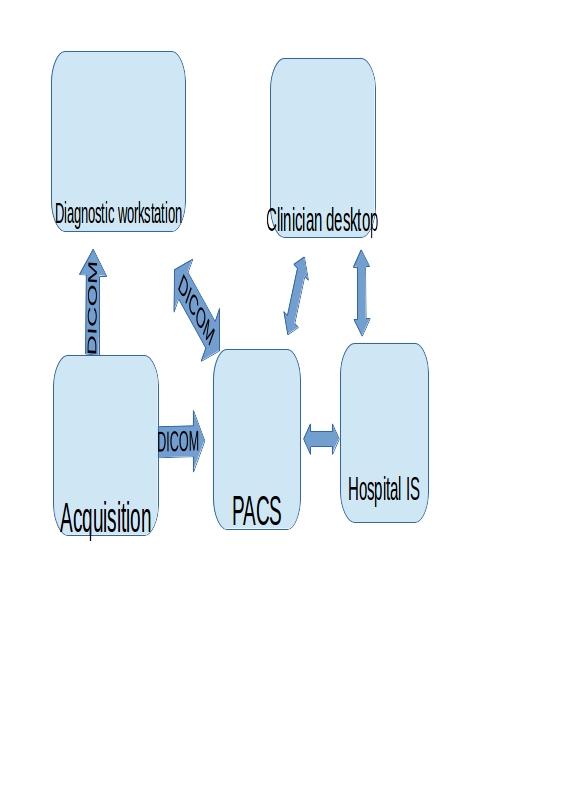
\includegraphics[width=0.8\textwidth, height=8cm]{chapter4/pacs.png}
    \caption{Typical workflow of medical image in hospital. Data acquisition is made by modalities (magnetic resonance, ultrasonography, X-ray radiography, etc.) and using DICOM format and protocol it can be directly transferred and visualized by diagnostic workstation. With metadata filled by an expert physician the image is stored in PACS. Other desktops within hospital can retrieve the image and review the report. The hospital information system may be involved in other workflows and communicate with other formats and standards (HL7,...)
    }
    \label{fig:pacs}
\end{figure}

As the data processed in hospital information systems contains sensitive information of real patients, these are protected and processing and storing is regulated by the national or international laws or agreements.
Development of telecomunication and network technologies a enabled telemedicine -- providing healthcare over remote distance. It requires to share and exchange  sensitive data of real patient among different helthcare providers and additionaly such data may be very valuable for further research. Security and encryption should be addressed and DICOM standard itself doesn't solve security issues appropriately, thus encyption during transferring the data over computer network must be ensured by other techniques.

In the Czech Republic, there exists several projects in production interconnecting different hospitals, clinics and other healthcare organization to exchange medical images. Project ePACS allows interconnecting each participant's PACS system via dedicated VPN channel to the central node and exchange of medical images are realized by routing the data flow from one VPN channel to the other\footnote{ePACS:\url{http://www.epacs.cz}, accessed January 2015}. Another approach is used in the project MEDIMED held by Masaryk University in Brno. Instead of dedicated VPN channel, they use  SSL encryption over standard TCP/IP communication and regional hospitals and healthcare providers are interconnected via the MEDIMED servers \cite{Slavicek2010,Zatloukal2012}.% \cite{Javornik2011,Zatloukal2012}.
In other countries, there were tested cross-border teleradiology in projects Baltic e-health, R-Bay and others \cite{Ross2010,Saliba2012}.
These projects are focused on sharing the medical images and other knowledge and information.

Storing the sensitive medical information is usually done in some trusted environment, e.g. in secured server or cluster owned by a trusted institution or within the hospital. In case of using distributed technologies, this lead to an idea to move and facilitate deployment of the grid services storing medical data to the institution which has been acknowledged to store them using e.g. pre-installed virtual machines as a sealed grid \cite{Kuba2007a}.

Additionaly for the research purposes an access to the wide range of medical images is needed for provenance, for research of new processing and diagnostic methods, etc.  DICOM records can be "deidentified" or anonymized for research purposes to protect sensitive personal data, but keep important information for research purposes. The Globus MEDICUS project published by Erberich et al.\cite{Erberich2006,Erberich2007} is based on Globus Toolkit middleware to federate clinical and research application via a grid-computing infrastructure. It  introduces a new DICOM Grid Interface Service for DICOM compliant devices and application based on Pixelmed Java DICOM Toolkit\footnote{\url{http://www.pixelmed.com/} accessed February 2015}. Currently the project is hibernated since 2008 and no further development was published\footnote{\url{https://dev.globus.org/wiki/Incubator/MEDICUS} accessed February 2015}. Similar effort was done with a project Medical Data Manager which uses gLite grid middleware by Duque, Montagnat et al.\cite{Duque,Montagnat2007} \footnote{\url{http://modalis.i3s.unice.fr/softwares/mdm/start} accessed February 2015} or MediGRID project by Krefting et al.{Krefting2009,Krefting2010}. These project focuses not only on sharing medical images and knowledge, but also on processing them using grid computing technologies\cite{Krefting2010}.

%When we look to the architecture of the systems of sharing medical images the problematic part within the point-to-multipoint architecture is the central part of the systems already in production e.g. in Czech Republic (MEDIMED, ePACS). This may become single point of failure and bottleneck.

To summarize this section, digital medical image acquisition, store, exchange and processing became common in the past years and is currently using distributed computing techniques. There are several efforts to implement medical data management within grid or cloud infrastructure for research purposes and integrate them with the production infrastructures. Security is solved by authentication, authorization mechanism as well as by encrypting the data and/or anonymizing them to keep minimal information useful for research. Thus there is another question, how easily the previously mentioned grid-based technologies can be integrated with current distributed systems used to integrate hospital PACS. The following section \ref{sec:methodsimages} describes methods used to integrate a pilot deployment of Globus MEDICUS with current regional system for exchanging medical images - MEDIMED. The realization and other promising particular results are described in section \ref{sec:resultsimages}.

\section{Methods to share medical images in grid}
\label{sec:methodsimages}

The integration strategies based on standard protocol integration and client server architecture is used to integrate Globus MEDICUS with some local PACS system. Globus MEDICUS \cite{Erberich2006,Erberich2007} implements a DICOM Grid Interface Service (DGIS) which in one side communicate using DICOM protocol, and implements other services which stores metadata and location of replicas of the data using standardized Globus toolkit middleware. DGIS behaves as a gateway to this grid infrastructure and is usually installed on the location of integrated third party system; hospital PACS, workstation PACS client or DICOM modality communicate with DGIS using DICOM protocol.
To present DICOM studies The integration strategy based on shared database or files can be used to present the DICOM studies via web portal. Additionally the web portal might generate specific DICOM queries to DGIS.

The paper \cite{kulhanek2009}  \emph{Processing of Medical Images in Virtual Distributed Environment} in Appendix \ref{app:a} published details about the integration of Globus MEDICUS instance with MeDiMed project with a conclusion that the integration via DICOM protocol is almost seamless. The paper \cite{Kulhanek2008Mefanet} presented additional portal integration with DICOMViewer, which can provide access to the DICOM studies available in the Globus MEDICUS infrastructure.


\section{Results}
\label{sec:resultsimages}
The pilot grid infrastructure was established in the location of First Faculty of Medicine, Charles University in Prague, Central Military Hospital in Prague and CESNET association. And the Globus Toolkit middleware and Globus MEDICUS implementation was installed on linux based virtual machines using XEN hypervisor providing pilot services to access this grid based PACS system.

